I dette afsnit vil vi først og fremmest undersøge nogle vigtige egenskaber ved $\mathbb{R}$, der er nødvendige for en stringent opbygning af integrationsteorien.
Derefter indfører vi grundlæggende teori om topologi for $\mathbb{R}$, som vi senere skal bruge til at definere kontinuitet samt grænseværdien for en funktion.\footnote{Afsnittet er baseret på \cite{Rudin1976}, s. 3-33, medmindre andet er angivet. Vi nøjes dog med at kigge på delmængder af $\mathbb{R}$, hvor Rudins bog behandler teorien mere generelt via metriske rum.}

\subsection{Supremum-egenskaben}%
  \label{sub:Supremum-egenskaben}

\begin{definition}[label=def:overtal]{Overtal, undertal, begrænset}{}
  Antag, at $A \subseteq \mathbb{R}$. 
  Hvis der eksisterer $y \in \mathbb{R}$ sådan at $x \leq y$ for alle $x \in A$, så siges $A$ at være opad begrænset, og $y$ kaldes et overtal for $A$. 

  Hvis der eksisterer $z \in \mathbb{R}$ sådan at $x \geq z$ for alle $x \in A$, så siges $A$ at være nedad begrænset, og $z$ kaldes et undertal for $A$. 

  Hvis $A$ både er opad begrænset og nedad begrænset, så kalder vi $A$ begrænset. 
\end{definition}

Imidlertid, kan det også være interessant at kunne sige noget om, hvorvidt et bestemt overtal er det mindste overtal og om et bestemt undertal er det største undertal.

\begin{definition}[label=def:sup]{Supremum, infimum}{}
  Antag, at $A \subseteq \mathbb{R}$. Et element $y \in \mathbb{R}$ kaldes supremum eller mindste overtal af $A$ og betegnes $\sup A$, hvis $y$ har følgende egenskaber:
  \begin{itemize}
    \item $y$ er et overtal for $A$.
    \item $y \leq z$ for alle overtal $z$ af $A$. 
  \end{itemize}
  Et element $\beta \in \mathbb{R}$ kaldes infimum eller største undertal af $A$ og betegnes $\inf A$, hvis $\beta$ har følgende egenskaber:
  \begin{itemize}
    \item $\beta$ er et undertal for $A$.
    \item $\beta \geq \alpha$ for alle undertal $\alpha$ af $A$. 
  \end{itemize}
\end{definition}

\begin{example}[label=exa:supinf]{Supremum og infimum af mængder}{}
  Betragt mængderne
  \[
  A=\{ a \in \mathbb{R}:a \leq 1 \}\quad \text{og} \quad B=\{ b \in \mathbb{R}: b>0 \}. 
  \] 
  Vi har så $\sup A=1$ og $\inf B=0$.
  Derudover er mængden $A$ ikke nedad begrænset og mængden $B$ er ikke opad begrænset. 
\end{example}

Bemærk, at $\sup A \in A$, hvor $\inf B \not\in B$.
Det næste eksempel viser, at en ikke-tom opad begrænset delmængde af $\mathbb{Q}$ kan have supremum, der ikke er i $\mathbb{Q}$. 

\begin{example}[label=exa:supQ]{\footnote{Eksemplet er baseret på \cite{Axler2024}, s. 9} Ikke-tom opad begrænset delmængde af $\mathbb{Q}$ uden supremum i $\mathbb{Q}$ }{}
  Lad
  \[
  A=\{ a \in \mathbb{Q}:a^2<2 \} 
  \] 
Antag, at $q \in \mathbb{Q}$.
Vi vil vise, at $q \neq \sup A$.
Siden $\sqrt{2} $ er irrational, så må vi have $q^2<2$ eller $q^2>2$. 

Hvis $q^2<2$, kan vi finde et element i $A$, der er lidt større end $q$.
Vælg
\[
  \delta=\frac{2-q^2}{5}.
\] 
Siden $q < \abs{\sqrt{2} }<2$ og $0<\delta \leq \frac{2}{5} <1$, så må der gælde, at $2q+\delta<5$. 
Vi har så 
\begin{equation*}
  \begin{split}
    \left(q + \delta \right)^2 &=q^2+\delta^2+2q \delta\\
    &=q^2+\left(2q+\delta \right) \cdot \delta \\
    &<q^2+5 \delta \\
    &=2.
  \end{split}
  \end{equation*}
  Med andre ord er $q + \delta $ altså et element i $A$, og $q \neq \sup A$.  

  Antag nu, at $q^2>0$ og $q>0$ (når $q \leq 0$ er det trivielt, at $q \neq \sup A$). 
  Lad 
  \begin{equation*}
  \begin{split}
   \alpha &=\frac{q^2-2}{2q}\\
  &=\frac{q}{2}-\frac{1}{q}\\
    &<b.
   \end{split}
  \end{equation*}
  Vi har så $0<\alpha <q$, og der gælder 
  \begin{equation*}
  \begin{split}
    \left(q-\alpha \right)^2&=q^2+\alpha ^2 - 2 q \alpha \\
    &<q^2-2q \alpha \\
    &=q^2-(q^2-2)\\
    &=2.
  \end{split}
  \end{equation*}
  Altså er $q- \alpha $ et overtal for $A$, hvilket vil sige, at $q \neq \sup A$. 
  Vi har nu vist, at mængden $A$ ikke har et supremum i $\mathbb{Q}$. 
\end{example}

Eksempel \ref{exa:supQ} motiverer den næste sætning, som vi her ikke vil bevise, da beviset er relativt langt og ikke interessant for vores foretagende.
Sætningen er dog en følge af måden, hvorpå $\mathbb{R}$ er konstrueret.\footnote{$\mathbb{R}$ kan konstrueres fra $\mathbb{Q}$ via Dedekind-snit. \cite{Rudin1976}, s. 17-21}

\begin{theorem}[label=theo:supremum-egenskab]{$\mathbb{R}$ har supremum-egenskaben}{}
  Antag, at $A \in \mathbb{R}$, $A \neq \emptyset$ og $A$ er opad begrænset. 
  Så eksisterer $\sup A \in \mathbb{R}$.
\end{theorem}

Denne egenskab ved $\mathbb{R}$ kaldes for supremum-egenskaben. 
Bemærk, at en alternativ tilgang her kunne være at definere $\mathbb{R}$ ud fra supremum-egenskaben og derefter bevise $\mathbb{R}$'s eksistens ved konstruktion.
Vi vil nu ud fra supremum-egenskaben af $\mathbb{R}$ vise, at $\mathbb{R}$ også må have infimum-egenskaben. 

\begin{theorem}[label=theo:infimum-egenskab]{$\mathbb{R}$ har infimum-egenskaben  }{}
  Antag, at $A \in \mathbb{R}$, $A \neq \emptyset$ og $A$ er nedad begrænset.
  Så eksisterer $\inf A \in \mathbb{R}$.
\end{theorem}
\begin{proof} 
  Lad 
  \[
  B=\{ b \in \mathbb{R} : b \leq a \text{ for alle } a \in A \}.
  \]  
  Så er $B$ mængden af alle undertal for $A$.
  Siden $A$ er nedad begrænset, så er $B$ ikke tom.
  Siden $A \neq \emptyset$, så er $B$ opad begrænset. 
  Fra supremum-egenskaben eksisterer da $\sup B \in \mathbb{R}$. 

  Per definition \ref{def:sup} har vi så, at $\sup B \leq a$ for alle $a \in A$ (fordi alle elementer af $A$ er overtal for $B$). 
  Siden $\sup B$ også er større end eller lig alle undertal for $A$, så må $\sup B=\inf A$. 
\end{proof}

\subsection{Topologi i $\mathbb{R}$}%
  \label{sub:Topologi i R}
Det skal bemærkes, at når vi arbejder med $\mathbb{R}$, så kan ordene \textit{punkt} og \textit{tal} bruges i flæng.
Begge ord referer i dette tilfælde til elementerne i $\mathbb{R}$.
  
\begin{definition}[label=def:omegn]{Omegn}{}
  Antag $p \in \mathbb{R}$. 
  Så er en omegn af et punkt $p$ en mængde 
  \[
  N_r(p)=\{ q \in \mathbb{R}:\abs{q-p} < r \}, \quad \text{ hvor }r \in \mathbb{R}^+. 
  \] 
  Tallet $r$ kaldes for radius af omegnen $N_r(p)$. 
\end{definition}
Med andre ord, er en omegn af et punkt $p$ mængden af alle punkter indenfor en given afstand fra $p$.
Ved en omegn i $\mathbb{R}$ (som vi lige har defineret) er der altså tale om et interval. 
Dette ses illustreret i \cref{fig:omegn}.
\begin{figure}[H]
\begin{center}
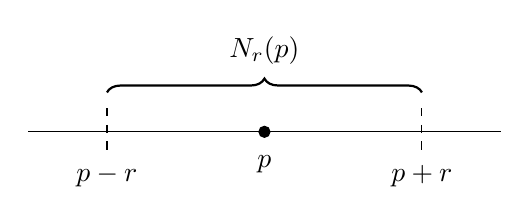
\begin{tikzpicture}
  \centering
    %\tikzstyle{point}=[circle,thick,draw=black,fill=black,inner sep=0pt,minimum width=4pt,minimum height=4pt]
    %\node [point] at (0,0) {};
    \filldraw[black] (0,0) circle (2pt) node[below=5pt]{$p$};
    \draw (-3,0) -- (3,0);
    \draw [dashed] (-2,0.3) -- (-2,-0.3) node[anchor=north]{$p-r$};
    \draw [dashed] (2,0.3) -- (2,-0.3) node[anchor=north]{$p+r$};
    \draw [decorate, decoration = {brace,amplitude=5pt}, thick] (-2,0.5) -- (2,0.5) node[midway,yshift=3.5ex]{$N_r(p)$};
    %\draw [decorate,decoration={brace,amplitude=5pt,mirror,raise=4ex}] (1,0) -- (5,0) node[midway,yshift=-3em]{Konvergenzbereich};
\end{tikzpicture}
\end{center}
  \caption{Illustration af en omegn $N_r(p)$}
\label{fig:omegn}
\end{figure}

\begin{definition}[label=def:åben]{Indre punkt, åben mængde }{}
  Antag, at $A \subseteq \mathbb{R}$. 
  Et punkt $p \in A$ kaldes et indre punkt af $A$, hvis der eksisterer en omegn $N_r(p)$ af $p$ sådan at $N_r(p) \subseteq A$. 

  Mængden $A$ er åben, hvis alle punkter i $A$ er indre punkter. 
\end{definition}

Som eksempel på åbne mængder, kan vi betragte omegne.

\begin{theorem}[label=theo:omegne_åbne]{Omegne er åbne}{}
  Alle omegne $N_r(p)$ af et punkt $p \in \mathbb{R}$ er åbne. 
\end{theorem}
\begin{proof} 
  Lad $q \in N_r(p)$ og $t=r-\abs{p-q} $.
  Så har vi $\abs{p-q} <r$, hvilket vil sige, at $t>0$.
  Fra trekantsuligheden har vi så, at der for alle $s \in N_t(q)$ gælder
  \begin{equation*}
  \begin{split}
    \abs{p-s} &\leq \abs{p-q} + \abs{q-s} \\
    &<\abs{q-p} + t \\
    &=r.
  \end{split}
  \end{equation*}
  Altså må $N_t(q)\subseteq N_r(p)$.
  Således er $N_r(p)$ en åben mængde.
\end{proof}

Ideen i beviset af sætning \ref{theo:omegne_åbne} ses illustreret i \cref{fig:omegne_åbne}.

\begin{figure}[H]
\begin{center}
\begin{tikzpicture}
  \centering
    \filldraw[black] (0,0) circle (2pt) node[below=3pt]{$p$};
    \filldraw[black] (3,0) circle (2pt) node[below=3pt]{$q$};
    \filldraw[black] (4.5,0) circle (2pt) node[below=3pt]{$s$};
    \draw (-8,0) -- (8,0);
    \draw [dashed] (-5,0.3) -- (-5,-0.3) node[anchor=north]{$p-r$};
    \draw [dashed] (5,0.3) -- (5,-0.3) node[align=left,anchor=north]{$p+r=q+t$};
    \draw [dashed] (1,0.3) -- (1,-0.3) node[anchor=north]{$q-t$};
    \draw [decorate, decoration = {brace,amplitude=10pt}, thick] (-5,0.5) -- (5,0.5) node[midway,yshift=5ex]{$N_r(p)$};
    \draw [decorate, decoration = {brace,amplitude=5pt,mirror}, thick] (1,-1) -- (5,-1) node[midway,yshift=-3.5ex]{$N_t(q)$};
    %\draw [decorate,decoration={brace,amplitude=5pt,mirror,raise=4ex}] (1,0) -- (5,0) node[midway,yshift=-3em]{Konvergenzbereich};
\end{tikzpicture}
\end{center}
  \caption{Ideen i beviset af sætning \ref{theo:omegne_åbne}}
\label{fig:omegne_åbne}
\end{figure}

\begin{definition}[label=def:fortætningspunkt]{Fortætningspunkt, isoleret punkt}{}
  Antag, at $A \subseteq \mathbb{R}$.
  Et punkt $p \in \mathbb{R}$ er et fortætningspunkt af mængden $A$, hvis alle omegne $N_r(p)$ indeholder et punkt $q \neq p$ i omegnen sådan at $q \in A$. 

Et punkt $s \in A$ kaldes et isoleret punkt, hvis det ikke er et fortætningspunkt af $A$. 
\end{definition}

Fra definitionen er det klart, at et fortætningspunkt af en mængde ikke nødvendigvis behøver være et element i mængden.
Dette tydeliggøres af det næste eksempel.

\begin{example}[label=exa:fortætningspunkter]{Fortætningspunkter af en mængde}{}
  Vi betragter mængden $B$ fra eksempel \ref{exa:supinf}. 
  Mængden af alle fortætningspunkter af $B$ må være $B'=B\, \cup\, \{ 0 \} $. 
For at se, hvorfor det er tilfældet, lad $p \in B'$.
  Så for enhver $r>0$ indeholder omegnen $N_r(p)$ et punkt $q=p+\frac{r}{2}$.
  Siden 
  \[
  p \geq 0 \iff p + \frac{r}{2} > 0 \iff q>0
  \] 
  så må vi have $q \in B$.
  Således må alle punkter i $B'$ være fortætningspunkter af $B$. 

  Omvendt, antag at $x \not\in B'$.
  Så har vi $x \in \{ x \in \mathbb{R}: x < 0 \} $.
  Vi kan så vælge $r=\abs{x} >0$, og det er klart at $N_r(x) \cap B = \emptyset$.
  Vi har nu vist, at $B'$ er mængden af alle fortætningspunkter af $B$.
\end{example}

Mere generelt gælder der faktisk, at hvis supremum og/eller infimum eksisterer for en delmængde af $\mathbb{R}$, så er de fortætningspunkter af mængden.

\begin{theorem}[label=theo:sup_fortætning]{Supremum og infimum er fortætningspunkter}{}
  Antag $A \subseteq \mathbb{R}$ og $A \neq \emptyset $.
  Hvis $A$ er opad begrænset, så er $\sup A$ et fortætningspunkt af $A$.
  Hvis $A$ er nedad begræset, så er $\inf B$ et fortætningspunkt af $A$. 
\end{theorem}
\begin{proof} 
  Antag, at $A$ er opad begrænset. 
  Så eksisterer $\alpha =\sup A$ (sætning \ref{theo:supremum-egenskab}).
  Antag, at $\alpha $ ikke er et fortætningspunkt af $A$. 
  Så eksisterer en omegn $N_r(\alpha )$ sådan at $N_r(\alpha ) \cap A=\emptyset $. 
  Men så er $\alpha - r$ et overtal for $A$, hvilket fører til modstrid.
  Altså må $\alpha $ være et fortætningspunkt af $A$. 

På tilsvarende måde kan man vise, at hvis $A$ er nedad begrænset, så er $\inf A$ et fortætningspunkt af $A$.  
\end{proof}

\begin{figure}[H]
\begin{center}
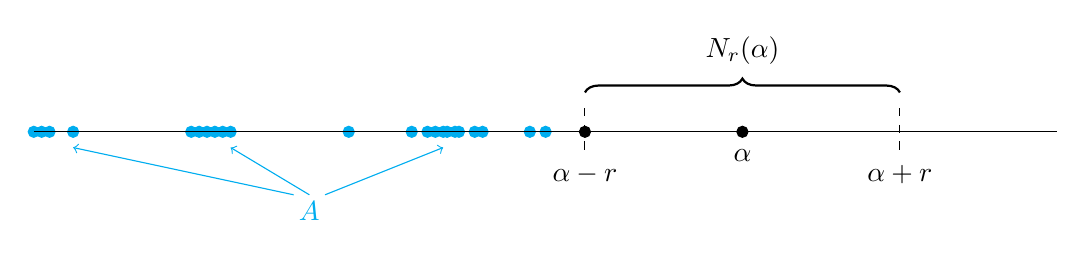
\begin{tikzpicture}
  \centering
    \filldraw[black] (0,0) circle (2pt);
    \filldraw[black] (2,0) circle (2pt) node[below=3pt]{$\alpha $};
    \filldraw[cyan] (-7,0) circle (2pt);
    \filldraw[cyan] (-6.9,0) circle (2pt);
    \filldraw[cyan] (-6.8,0) circle (2pt);
    \filldraw[cyan] (-6.5,0) circle (2pt);
    \filldraw[cyan] (-5,0) circle (2pt);
    \filldraw[cyan] (-4.9,0) circle (2pt);
    \filldraw[cyan] (-4.8,0) circle (2pt);
    \filldraw[cyan] (-4.7,0) circle (2pt);
    \filldraw[cyan] (-4.6,0) circle (2pt);
    \filldraw[cyan] (-4.5,0) circle (2pt);
    \filldraw[cyan] (-3,0) circle (2pt);
    \filldraw[cyan] (-2,0) circle (2pt);
    \filldraw[cyan] (-2.2,0) circle (2pt);
    \filldraw[cyan] (-1.9,0) circle (2pt);
    \filldraw[cyan] (-1.8,0) circle (2pt);
    \filldraw[cyan] (-1.75,0) circle (2pt);
    \filldraw[cyan] (-1.65,0) circle (2pt);
    \filldraw[cyan] (-1.6,0) circle (2pt);
    \filldraw[cyan] (-1.4,0) circle (2pt);
    \filldraw[cyan] (-1.3,0) circle (2pt);
    \filldraw[cyan] (-0.5,0) circle (2pt);
    \filldraw[cyan] (-0.7,0) circle (2pt);
    \draw[cyan] (-3.5,-1) node {$A$};
    \draw[cyan, ->] (-3.7,-0.8) -- (-6.5,-0.2);
    \draw[cyan, ->] (-3.5,-0.8) -- (-4.5,-0.2);
    \draw[cyan, ->] (-3.3,-0.8) -- (-1.8,-0.2);
    \draw (-7,0) -- (6,0);
    \draw [dashed] (4,0.3) -- (4,-0.3) node[align=left,anchor=north]{$\alpha +r$};
    \draw [dashed] (0,0.3) -- (0,-0.3) node[anchor=north]{$\alpha -r$};
    \draw [decorate, decoration = {brace,amplitude=5pt}, thick] (0,0.5) -- (4,0.5) node[midway,yshift=3.5ex]{$N_r(\alpha )$};
    %\draw [decorate,decoration={brace,amplitude=5pt,mirror,raise=4ex}] (1,0) -- (5,0) node[midway,yshift=-3em]{Konvergenzbereich};
\end{tikzpicture}
\end{center}
  \caption{Antagelsen om, at $\alpha $ ikke er et fortætningspunkt fører til modstrid }
\label{fig:sup_fortætning}
\end{figure}


Faktummet, at et fortætningspunkt af en mængde ikke nødvendigvis er et element i mængden (hvilket vi så i eksempel \ref{exa:fortætningspunkter}), motiverer den næste definition.

\begin{definition}[label=def:lukket]{Lukket mængde }{}
  En mængde $A \subseteq \mathbb{R}$ er lukket, hvis den indeholder alle sine fortætningspunkter. 
\end{definition}

Vi vil nu bevise det intuitive resultat, at komplementærmængden til en åben mængde er lukket, og vice versa.
Bemærk, at nogle benytter notationen $\overline A$ til at denotere afslutningen af $A$ (foreningsmængden af $A$ og mængden af alle dens fortætningspunkter), hvor vi her bruger $\overline A$ til at denotere komplementærmængden til $A$.

\begin{theorem}[label=theo:åben_lukket_komp]{Mængde er lukket præcis når dens komplementærmængde er åben}{}
  En mængde $A \in \mathbb{R}$ er lukket hvis og kun hvis dens komplementærmængde $\overline A$ er åben. 
\end{theorem}
\begin{proof} 
  Antag først, at $A$ er lukket.
  Så er alle $x \in \overline A$ ikke fortætningspunkter af $A$, og der eksisterer en omegn $N_r(x)$ sådan at $A \cap N_r(x)=\emptyset$. 
  Det vil sige, at $N_r(x) \subseteq \overline A$, og $x$ er derfor et indre punkt af $\overline A$.
  Således er $A$ åben. 

  Omvendt, antag at $\overline A$ er åben, og lad $p$ være et fortætningspunkt af $A$. 
  Så indeholder alle omegne $N_r(p)$ et punkt $q \in A$, og $p$ er derfor ikke et indre punkt af $\overline A$.
  Siden $\overline A$ er åben, så må $p \in A$.
  Altså indeholder $A$ alle sine fortætningspunkter og må være lukket. 
\end{proof}

